\section{definisi}
Unshielded twisted pair (UTP) adalah jenis kabel tembaga mana-mana yang digunakan pada kabel telepon dan jaringan area lokal (LAN).
Dalam operasi garis seimbang, kedua kabel membawa sinyal sama dan berlawanan, dan tujuan mendeteksi perbedaan antara keduanya. Hal 
ini dikenal sebagai modetransmission differential. Sumber kebisingan mengenalkan sinyal ke kabel dengan menggabungkan medan listrik 
atau medan magnet dan cenderung berpasangan dengan kedua kabel dengan sama. Kebisingan tersebut menghasilkan sinyal mode umum yang 
dibatalkan pada receiver saat sinyal perbedaan diambil. Metode ini mulai gagal saat sumber suara dekat dengan kabel sinyal; kawat 
yang lebih dekat akan berpasangan dengan noise lebih kuat dan penolakan mode umum pada penerima akan gagal untuk menghilangkannya. 
Masalah ini terutama terlihat pada kabel telekomunikasi dimana pasangan kabel yang sama saling berdekatan satu sama lain selama 
bermil-mil. Satu pasang bisa menyebabkan crosstalkin lain dan itu aditif sepanjang kabel. Memutar pasang counter efek ini seperti 
pada masing-masing setengah memutar kawat yang terdekat dengan sumber noise yang dipertukarkan. Menyediakan sumber yang mengganggu 
tetap seragam, atau hampir, lebih dari jarak satu putaran, kebisingan yang diinduksi akan tetap umum. Diferensial sinyal juga mengurangi 
radiasi elektromagnetik dari kabel, bersamaan dengan atenuasi yang terkait sehingga memungkinkan jarak yang lebih jauh antara pertukaran. 
Tingkat twist (juga disebut pitch of twist, biasanya didefinisikan dalam twists per meter) merupakan bagian dari spesifikasi untuk jenis 
kabel tertentu. Bila pasangan di dekatnya memiliki tingkat twist yang sama, konduktor yang sama dari pasangan yang berbeda dapat berulang 
kali berbohong satu sama lain, dan sebagian membatalkan manfaat dari mode diferensial. Untuk alasan ini biasanya ditentukan bahwa, setidaknya 
untuk kabel yang mengandung sejumlah kecil pasang, tingkat twist harus berbeda. Berbeda dengan twisted pair terlindung atau tergoda (biasanya 
perisai kabel F / UTP atau S / FTP), kabel UTP (unshielded twisted pair) tidak dikelilingi oleh perisai. UTP adalah tipe kabel utama untuk 
telepon dan sangat umum untuk jaringan komputer, terutama sebagai kabel patch atau koneksi jaringan sementara karena tingginya fleksibilitas kabel.

	contoh gambar utp dan stp \ref{utp_stp.stp}
	\begin{figure}[ht]
		\centerline{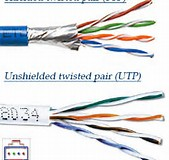
\includegraphics[width=1\textwidth]{figures/utp_stp.jpg}}
		\caption{gambar utp dan stp.}
		\label{utp_stp}
	\end{figure}

\subsection{sejarah}
Telepon paling awal menggunakan jalur telegraf, atau kawat kisi-kisi belakang kawat tunggal. Pada tahun 1880-an, trem listrik dipasang di banyak kota, 
yang menyebabkan kebisingan masuk ke sirkuit ini. Tuntutan hukum yang tidak layak, perusahaan telepon beralih ke sirkuit seimbang, yang memiliki manfaat 
sampingan pengurangan emisi, sehingga meningkatkan jangkauan. Karena distribusi tenaga listrik menjadi lebih umum, ukuran ini terbukti tidak memadai. 
Dua kabel, digantung di kedua sisi palang palang di tiang listrik, berbagi rute dengan jalur listrik. Dalam beberapa tahun, meningkatnya penggunaan 
listrik kembali membawa peningkatan interferensi, sehingga para insinyur merancang sebuah metode yang disebut transposisi kawat, untuk membatalkan 
interferensi tersebut. Dalam transposisi kawat, posisi pertukaran kabel setiap beberapa tiang. Dengan cara ini, kedua kabel akan menerima similarEMI 
dari kabel listrik. Ini merupakan implementasi awal memutar, dengan tingkat twist sekitar empat twists perkilometre, atau enam per mil. Garis seimbang 
kawat terbuka semacam itu dengan transposisi periodik masih bertahan sampai sekarang di beberapa daerah pedesaan. Kabel twisted-pair diciptakan oleh 
Alexander Graham Bell pada tahun 1881. [3] Pada tahun 1900, jaringan saluran telepon Amerika secara keseluruhan adalah twisted pair atau open wire dengan 
transposisi untuk mencegah gangguan. Saat ini, sebagian besar dari jutaan pasang twisted pair di dunia adalah sambungan telepon rumah, yang dimiliki oleh 
perusahaan telepon, digunakan untuk layanan suara, dan hanya ditangani atau bahkan dilihat oleh pekerja telepon. Unshielded twisted pair (UTP) kabel 
ditemukan di banyak jaringan Ethernet dan sistem telepon. Bagian khas dari warna-warna ini (putih / biru, biru / putih, putih / oranye, oranye / putih) 
muncul di sebagian besar kabel UTP. Kabel biasanya dibuat dengan kabel tembaga yang diukur pada 22 atau 24 American Wire Gauge (AWG), [4] dengan insulasi 
berwarna yang biasanya dibuat dari isolator seperti polietilen atau FEP dan total paket yang dilapisi jaket apolyetilena. Untuk kabel telepon luar kota 
yang berisi ratusan atau ribuan pasang, kabelnya terbagi menjadi beberapa paket kecil namun identik. Setiap bundel terdiri dari pasangan twisted yang 
memiliki tingkat twist berbeda. Bundel pada gilirannya dipelintir bersama untuk membuat kabel. Pasangan yang memiliki tingkat twist yang sama di dalam 
kabel masih bisa mengalami beberapa derajatcrosstalk. Pasangan kawat dipilih dengan hati-hati untuk meminimalkan crosstalk dalam kabel besar. Kabel 
twisted pair unshielded dengan tingkat twist yang berbeda Kabel UTP juga merupakan kabel yang paling umum digunakan dalam jaringan komputer. ModernEthernet, 
standar jaringan data yang paling umum, bisa menggunakan kabel UTP. Kabel twisted pair sering digunakan pada jaringan data untuk koneksi jarak pendek dan 
menengah karena biaya yang relatif lebih rendah dibandingkan kabel serat optik dan koaksial. UTP juga menemukan peningkatan penggunaan dalam aplikasi video, 
terutama di kamera keamanan. Banyak kamera termasuk keluaran UTP dengan terminal kecil; Bandwidth kabel UTP telah meningkat agar sesuai dengan sinyal baseband 
dari televisi. Karena UTP adalah saluran transmisi yang seimbang, balun diperlukan untuk terhubung ke peralatan yang tidak seimbang, misalnya menggunakan 
konektor BNC dan dirancang untuk kabel koaksial.

\subsection {Karakter Kabel}
CAT1 biasanya digunakan untuk kabel telepon. Jenis kabel ini tidak mampu mendukung lalu lintas jaringan komputer dan tidak terpelintir. CAT1is juga digunakan 
oleh perusahaan telco yang menyediakan layanan ISDN dan PSTN. Dalam kasus seperti ini, pemasangan kabel antara situs pelanggan dan jaringan telco dilakukan 
dengan menggunakan kabel tipe CAT 1.

CAT2, CAT3, CAT4, CAT5 / 5e, CAT6 dan CAT 7 adalah spesifikasi kawat jaringan. Jenis kawat ini bisa mendukung jaringan komputer dan lalu lintas telepon. CAT2 
banyak digunakan untuk jaringan token ring, mendukung kecepatan hingga 4 Mbps. Untuk kecepatan jaringan yang lebih tinggi (100 Mbps atau lebih tinggi) CAT5e 
harus digunakan, namun untuk persyaratan kecepatan 10 Mbps yang hampir punah, CAT3 sudah cukup.

Kabel CAT3, CAT4 dan CAT5 sebenarnya adalah 4 pasang kawat tembaga twisted dan CAT5 memiliki tikungan lebih banyak per inci dari pada CAT3 sehingga dapat 
berjalan pada kecepatan yang lebih tinggi dan panjang yang lebih besar. Efek "twist" dari masing-masing pasangan di kabel memastikan adanya gangguan yang 
muncul / diangkat pada satu kabel dibatalkan oleh pasangan kabel yang memutar di sekitar kabel awal. CAT3 dan CAT4 keduanya digunakan untuk jaringan Token 
Ring - di mana CAT 3 dapat memberikan dukungan maksimal 10Mbps, sementara CAT4 mendorong batas hingga 16Mbps. Kedua kategori tersebut memiliki batas 100 meter.

Kabel CAT5 yang lebih populer kemudian digantikan oleh spesifikasi CAT5e yang memberikan spesifikasi crosstalk yang lebih baik, yang memungkinkannya untuk 
mendukung kecepatan hingga 1Gbps. CAT5e adalah spesifikasi kabel yang paling banyak digunakan di seluruh dunia dan tidak seperti kabel kategori yang 
mengikutinya, sangat pemaaf saat panduan penghentian kabel dan penyebaran tidak terpenuhi.

Kabel CAT6 pada awalnya dirancang untuk mendukung gigabit Ethernet, walaupun ada standar yang memungkinkan transmisi gigabit melalui kabel CAT5e. Serupa 
dengan kabel CAT5e, namun ada pemisah fisik antara keempat pasang untuk mengurangi gangguan elektromagnetik. CAT6 mampu mendukung kecepatan 1Gbps untuk 
panjang hingga 100 meter, dan 10Gbps juga didukung untuk panjang hingga 55 meter.

Saat ini, sebagian besar instalasi kabel baru menggunakan CAT6 sebagai standar, namun penting untuk dicatat bahwa semua komponen kabel (jack, panel patch, 
kabel patch dll) harus dilindungi CAT6 dan ekstra hati-hati harus diberikan pada penghentian kabel yang tepat. .

Pada tahun 2009, CAT6A diperkenalkan sebagai kabel spesifikasi yang lebih tinggi, menawarkan imunisasi yang lebih baik pada gangguan crosstalk dan elektromagnetik.

	contoh gambar utp \ref{utp}
	\begin{figure}[ht]
		\centerline{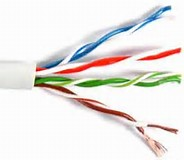
\includegraphics[width=1\textwidth]{figures/utp.jpg}}
		\caption{gambar utp.}
		\label{utp}
	\end{figure}
	
	contoh gambar stp \ref{stp}
	\begin{figure}[ht]
		\centerline{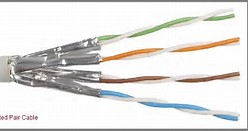
\includegraphics[width=1\textwidth]{figures/stp.jpg}}
		\caption{gambar stp.}
		\label{stp}
	\end{figure}
	
\subsection{Keuntungan}
1. Suara listrik masuk atau keluar dari kabel bisa dicegah.
2. Bentuk kabel termurah yang tersedia untuk keperluan jaringan.
3. Mudah untuk menangani dan menginstal.

\subsection{Kekurangan}
1. Deformasi: Kerentanan twisted pair terhadap interferensi elektromagnetik sangat bergantung pada skema twisted pair (kadang dipatenkan oleh produsen) 
tetap terjaga selama pemasangan. Akibatnya, kabel twisted pair biasanya memiliki persyaratan ketat untuk tegangan tarik maksimal serta radius tikungan 
minimum. Kerapihan kabel twisted pair ini membuat praktik pemasangan menjadi bagian penting untuk memastikan kinerja kabel.
2. Delay condong: pasangan yang berbeda dalam kabel memiliki penundaan yang berbeda, karena tingkat twist berbeda yang digunakan untuk meminimalkan crosstalk 
di antara pasangan. Hal ini dapat menurunkan kualitas gambar saat beberapa pasang digunakan untuk membawa komponen sinyal video. Kabel miring rendah tersedia 
untuk mengurangi masalah ini.
3. Ketidakseimbangan: perbedaan antara kedua kabel pada pasangan dapat menyebabkan kopling antara mode umum dan mode diferensial. Diferensial terhadap konversi
mode umum menghasilkan arus mode umum yang dapat menyebabkan interferensi eksternal dan dapat menghasilkan sinyal mode umum pada pasangan lainnya. Mode umum 
untuk konversi mode diferensial dapat menghasilkan sinyal mode diferensial dari interferensi mode umum dari pasangan lain atau sumber eksternal. 
Ketidakseimbangan dapat disebabkan oleh asimetri antara dua konduktor pasangan satu sama lain dan dalam hubungan dengan kabel lain dan perisai. Beberapa 
sumber asimetri adalah perbedaan diameter konduktor dan ketebalan insulasi. Dalam jargon telepon, mode umum disebut longitudinal dan mode diferensial 
disebut metalik.

\subsection{KARAKTERISTIK UTP}

Karakteristik UTP sangat bagus dan memudahkan untuk bekerja dengan, menginstal, memperluas dan memecahkan masalah dan kita akan melihat skema pengkabelan yang 
berbeda yang tersedia untuk UTP, bagaimana membuat kabel UTP langsung, peraturan untuk operasi yang aman dan banyak hal keren lainnya!
Kategori 1/2/3/4/5/6/7 - spesifikasi untuk jenis kawat tembaga (kebanyakan kawat telepon dan jaringan adalah tembaga) dan jack. Angka (1, 3, 5, dll) 
mengacu pada revisi spesifikasi dan secara praktis mengacu pada jumlah tikungan di dalam kawat (atau kualitas koneksi dalam jack).



\subsection{ATP terhadap UTP}
ATP dilepaskan dari sebagian besar jenis sel dan berfungsi sebagai molekul pensinyalan ekstraselular melalui aktivasi anggota dua keluarga besar reseptor 
P2X dan P2Y. Meskipun tiga reseptor P2Y mamalia telah dikloning yang diaktifkan secara selektif oleh nukleotida urida, demonstrasi langsung pelepasan UTP 
seluler belum dilaporkan. Studi farmakologi reseptor P2Y4 yang diekspresikan pada sel astrocytoma manusia 1321N1 mengindikasikan bahwa reseptor ini diaktifkan 
oleh UTP namun tidak oleh ATP. Stimulasi mekanis sel 1321N1 juga menghasilkan pelepasan molekul yang secara nyata mengaktifkan reseptor P2Y4 yang dinyatakan. 
Nukleotida ini terbukti UTP dengan dua cara. Pertama, analisis kromatografi cair kinerja tinggi medium dari sel 3321] yang dilepaskan oleh O3PO4 memuat 1321N1 
sehingga stimulasi mekanis menghasilkan peningkatan besar pada spesies radioaktif yang digerakkan bersama dengan UTP asli. Spesies ini terdegradasi oleh 
inkubasi dengan apyrase pyrophosphohydrolase nonspesifik atau dengan heksokinase dan secara khusus hilang melalui inkubasi dengan enzim UTP-glukosa 
pirofosforilase UDP. Kedua, uji sensitif yang mengkuantifikasi massa UTP pada konsentrasi nanomolar rendah dirancang berdasarkan spesifisitas nukleotida dari 
pirofosforilase UDP-glukosa. Dengan menggunakan uji ini, rangsangan mekanis sel 1321N1 terbukti menghasilkan peningkatan tingkat UTP medium dari 2,6 menjadi 
36,4 pmol / 106cells dalam 2 menit. Peningkatan ini disejajarkan dengan augmentasi serupa dari tingkat ATP ekstraselular. Metode quenching fluoresensi 
berbasis calcein digunakan untuk memastikan bahwa tidak ada peningkatan kadar nukleotida medium yang dapat dipertanggungjawabkan dengan lisis sel. Secara 
bersamaan, hasil ini secara langsung menunjukkan pelepasan UTP yang diinduksi secara mekanis dan menggambarkan kopling yang efisien dari pelepasan ini ke 
aktivasi reseptor P2Y4.

\section{CARA MEMBUAT KABEL ETHERNET}

Pembelian kabel Ethernet bisa sangat mahal dan panjang pra-dibuat tidak selalu panjang yang Anda butuhkan. Membuat kabel Ethernet mudah dengan sekotak kabel 
Ethernet kategori 5e dan konektor RJ-45 yang dilekatkan pada ujung yang dipotong dari panjang kabel yang Anda inginkan.
Kabel Ethernet Massal - Kategori 5e atau CAT5e
(Anda juga dapat menggunakan kabel Kategori 6 atau CAT6 yang memiliki spesifikasi kinerja lebih tinggi dan sekitar 20% lebih mahal dari CAT5e.)

Konektor Konter RJ45 Massal untuk CAT-5e atau Konektor Konter RJ45 Massal untuk CAT-6
Alat crimping RJ-45
Standard Ethernet Ada dua jenis kabel Ethernet yang bisa Anda buat, Straight Through dan Crossover.
Straight Through kabel Ethernet adalah kabel standar yang digunakan untuk hampir semua tujuan, dan sering disebut "kabel patch". Sangat disarankan Anda 
menduplikat urutan warna seperti yang ditunjukkan di sebelah kiri. Perhatikan bagaimana pasangan hijau tidak berdampingan sama seperti pasangan lainnya. 
Konfigurasi ini memungkinkan pengoperasian kabel lebih lama.
Kabel crossover
KABEL CROSSOVER - Tujuan dari kabel Crossover Ethernet adalah menghubungkan secara langsung satu komputer ke komputer lain (atau perangkat) tanpa melalui 
router, switch atau hub.
Inilah cara membuat kabel standar:
Potong selubung plastik sekitar 1 inci (2,5 cm) dari ujung kabel potong. Alat crimping memiliki pisau cukur yang akan melakukan trik dengan latihan.
Bersantai dan pasang warna yang sama.
Jepit kabel antara jari Anda dan luruskan mereka seperti yang ditunjukkan. Tata warna penting untuk mendapatkan yang benar.
Gunakan gunting untuk memotong lurus ke 8 kabel untuk mempersingkatnya menjadi 1/2 inci (1,3 cm) dari lengan potong sampai ujung kabel.
Dengan hati-hati tekan semua 8 kabel berwarna yang tidak dilapisi ke dalam konektor. Perhatikan posisi lengan plastik biru. Perhatikan juga bagaimana kabelnya
 sampai ke ujungnya.
Sebuah pemandangan dari atas. Semua kabel ada di dalamnya. Tidak ada kabel pendek.
 

\\Crimping Ethernet
hati-hati letakkan konektor ke Ethernet Crimper dan masuk ke pegangan dengan erat. Tab splicing tembaga pada konektor akan menembus masing-masing dari delapan 
kabel. Ada juga tab pengunci yang menahan lengan plastik biru agar sesuai dengan kompresi yang ketat. Bila Anda melepaskan kabel dari crimper, ujungnya siap 
digunakan.
Untuk kabel "Straight Through" standar, ulangi semua langkah dan tatanan warna kawat di ujung kabel yang lain. Untuk kabel cross-over, ujung lainnya akan 
memiliki tatanan warna yang berbeda seperti gambar crossover diatas.
Tester Kabel Ethernet
Pastikan untuk menguji kabel sebelum memasangnya. Tester kabel Ethernet murah melakukan ini dengan cukup baik

\cite{caniggia2003common}
\cite{jakovljevic2008common}
\cite{ueda2011transmission}
\cite{gagnon2002cable}
\cite{ueda2011transmission}
\cite{gomez2003receive}
\cite{blouin2002cross}